\documentclass[memoire.tex]{subfiles}
\begin{document}
\chapter{Etat de l'art du clustering}
Le Terme clustering fait référence au concept de classification non supervisée faisant elle même partie d'une plus grande famille qui est l'apprentissage non supervisé. A l'inverse de l'apprentissage supervisé qui nécessite des données déjà segmentées, le clustering vise quant à lui à déterminer une segmentation du jeu de données étudié. Dans ce cas, l'intervention humaine n'est pas nécessaire étant donné  que l'ordinateur détermine les différentes segmentations sans l'apport de variables cibles fournies à l'algorithme.
L'analyse de cluster permet donc d'identifier des groupes de données relativement homogènes sur la base de leur similarité pour des caractéristiques données ce qui dans notre cas peut par exemple être le type d'emploi occuper en fonction des filières suivies par d'anciens étudiants. Cependant analyser différents profils d'individus peut représenter des difficultés techniques importantes, c'est pourquoi cette première section du document présentera les différentes solutions possibles pouvant apporter une réponse à cette difficulté de catégorisation des parcours.
\section{La préparation des données}
Lorsqu'une segmentation basée sur des clusters est utilisée, il existe plusieurs formes de préparations de données pouvant aider à la formation des différents segments. 
\subsection{La Transformation des variables}
Il existe deux types de transformation : \begin{itemize}
\item La modification de la portée des variables connues
\item{La modification de la forme de distribution}
\end{itemize}
L'utilisation de la standardisation est motivée par le fait que l'analyse de cluster implique une étude implicite du poids des objets afin de pouvoir se concentrer sur ceux possédant une variance plus élevée. Les méthodes de standardisation les plus communes sont les suivantes \cite{ref9} : \begin{itemize}
\item Multiplication de chaque variable par une différente constante.
\item Utilisation des techniques de réduction de dimensions, qui est un processus visant à réduire le nombre de variables aléatoires afin d'obtenir un jeu de variables principal.
\item Multiplier chaque variables par une différente constante afin que chacune d'entre elles aient une portée commune.
\end{itemize}
La modification de la distribution quant à elle est motivée par les mêmes problématiques que dans d'autres secteurs ayant recours aux statistiques qui sont d'extrêmes variations par rapport à ce qui est considéré "normal" dans le cas étudié. Celles-ci entrainent des analyses pouvant induire en erreur. Par conséquent lorsque le poids des variables est modifié le but est d'identifier et supprimer leur longue traine qui correspond à un nombre de variables possédant des valeurs très supérieures ou inférieures à la moyenne.

\section{La mesure de distance}
Le choix de la méthode de mesure de distance est une étape critique pour les méthodes de clustering, son choix ayant une très forte influence sur le résultat final. En effet, la méthodologie choisie définira comment les similarités de deux éléments sont calculées et influera par conséquent sur la forme des clusters également. Les deux méthodes les plus communes de mesure sont la distance Euclidienne illustrée par la formule suivante (figure1.1) : 

	\begin{figure}[h!]
		\centerline{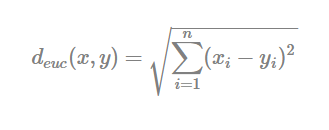
\includegraphics[scale=0.8]{img/euclidienne_distance.png}}
		\caption{Distance Euclidienne}
	\end{figure}
Dans cette méthode, la distance est calculée en effectuant le carré de la somme des carrés des distances entre les variables répondant à un critère donné.\\
La seconde méthode communément utilisée est la distance de Manhattan, appelée également "taxi-distance". Celle-ci, pour un point A et B de coordonnées respectives ($X_{a}$,$Y_{a}$) et ($X_{b}$,$Y_{b}$) est définie de la façon  suivante :\\
\begin{center}
$d(A,B) = [X_{b} - X_{a}] + [Y_{b} - Y_{a}]$\\
\end{center}
À l'inverse de la méthode euclidienne qui pourrait être influencée par des valeurs inhabituelles, le calcul de la distance de Manhattan va s'effectuer selon la différence moyennes entre les dimensions. La présence de valeurs aberrantes impactera le résultat de façon réduite étant donné qu'elles ne seront pas élevées au carré contrairement à la méthode euclidienne, ce qui fait que cette méthode aura tendance à donner le même type de résultat.
\newpage
\section{Les méthodes de clustering}
		\subsection{Le clustering hiérarchique}
Parmis les différents types de clustering existant \cite{ref4}, le premier étudié sera le clustering hiérarchique. Très utilisé comme outil d'analyse de données, l'idée principale de cette méthode est de construire un arbre binaire fusionnant de façon successive les groupes de points similaires. L'un des avantages de cette façon de faire  est tout d'abord l'apport de l'arbre qui permet d'avoir une vision globale des données traitées. De plus, cette méthodologie possède ses propres outils de visualisation qui sont le dendrogramme et la classification double. Le dendrogramme permet d'illustrer l'arrangement des clusters (figure 1.2)\cite{ref8} :
\begin{itemize}
\item la racine de l'arbre est formée par un cluster contenant l'ensemble des objets.
\item chaque nœud de l'arbre constitue un cluster.
\item l'union des objets des nœuds fils correspond aux objets présents dans le nœud racine.
\item les paliers sont indexés en fonction de l'ordre de construction.
\end{itemize}

 Tandis que la classification double est une technique d'exploration de données non-supervisée permettant de segmenter simultanément les lignes et les colonnes d'une matrice. L'autre avantage du clustering hiérarchique est sa facilité d'implémentation dans des algorithmes tel que K-Means en plus de fournir une représentation graphique comme dit précédemment. Afin d'établir un arbre hiérarchique, le processus de clustering à recours à deux méthodes qui sont la méthode agglomérative et la méthode divisive.\\ Un regroupement agglomératif traite chaque objet comme un seul élément qui à chaque étape de l'algorithme est fusionné avec un second objet présentant le plus de similarités en un nouveau cluster de plus grande taille. Ce processus est répété jusqu'à que ce que tous les points soient membre d'un seul et même cluster. À l'inverse d'un regroupement agglomératif qui utilise une approche "bottom-up", les algorithmes divisifs utilisent une approche "top-down". Ces algorithmes débutent ainsi leur traitement à partir de la racine de l'arbre ou tous les objets sont regroupés en un seul cluster. À chaque itération les cluster les plus hétérogènes sont divisés en deux jusqu'à ce que l'ensemble des objets fassent partie de leur propre cluster. Toutefois sa complexité le rend inefficace sur de larges jeux de données \cite{ref7}. De plus, la première injection de données ainsi que l'ordre de celles-ci  à un fort impact sur le résultat final. En outre, il n'est pas possible de défaire ou modifier les étapes précédentes du traitement, c'est-à-dire qu'une fois une instance assignées à un cluster, il n'est plus possible de la déplacée pour effectuer d'éventuelles modifications ou corrections \cite{ref5}. Dans notre cas la base de CV utilisée n'étant pas de taille importante le clustering hiérarchique reste une méthode applicable. Cependant la problématique à résoudre est la gestion des filières intégrant plusieurs domaines tel que la filière MIASHS de Nanterre qui possède une dimension mathématique et une informatique. Les données étant représentées sous \textit{forme d'arbre cela entrainerait une répétition au niveau des résultats.
	\begin{figure}[h!]
		\centerline{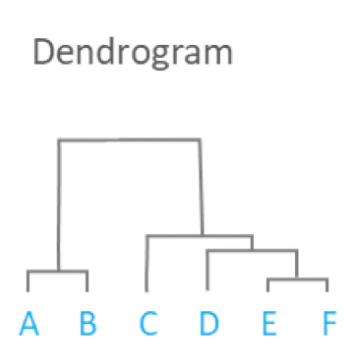
\includegraphics[scale=0.8]{img/hierarchical_clustering.png}}
		\caption{Exemple de dendrogramme}
	\end{figure}}
	
\newpage
\subsection{Le clustering par partitionnement}
Le clustering par partionnement contrairement au clustering hiérarchique qui utilise un arbre afin de représenter les différents groupe de données va classifier les différents objets en groupe en fonction de leur similarités. Cependant ce mode de fonctionnement pause un problème concernant le choix de la "bonne représentation" en fonction d'un critère choisi, le but devient alors de rechercher une représentation optimale de son critère à travers plusieurs itérations.\cite{ref8} L'algorithme le plus utilisé pour ce type de méthode est K-means qui sera présenté dans la suite de ce document. Dans le cas du clustering par partitionnement, il existe une sous-catégorie nommée le partitionnement flou. Celle-ci à recours à une autre version de l'algorithme k-means appelée \textit{Fuzzy k-means} ou k-moyennes flou. Cet algorithme cherche à minimiser la fonction illustrée par la figure 1.3.
	\begin{figure}[h!]
		\centerline{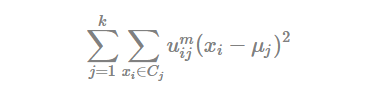
\includegraphics[scale=0.8]{img/fuzzy_algo.png}}
		\caption{Fonction objectif de Fuzzy k-means}
	\end{figure}
Dans la figure ci-dessus, \begin{itemize}
\item $u_{ij}$ est le degré selon lequel une observation $x_{i}$ appartient à un cluster $c_{j}$.
\item $\mu_j$ est le centre d'un cluster $j$.
\item $m$ est le "fuzzifier".\\
Contrairement aux méthodes de clustering dites dures, lorsque l'on a recours au clustering flou, il est possible que des données fassent partie de plusieurs clusters. De plus, l'appartenance d'un object à un cluster est ici décidé par la proximité entre le centre du cluster traité et l'objet en question. \cite{ref13} Cet algorithme reste toutefois soumis aux mêmes restrictions que l'agorithme k-means classique dans le fait qu'il requiert de spécifier le nombre de clusters souhaités.
\end{itemize}


\section{Les autres types de clustering}
\subsection{Le clustering basé sur des mélanges de modèles}
Cette approche est adoptée lors de l'utilisation d'apprentissage automatique et au traitement de données manquantes ou cachées, par rapport à d'autes approches basées sur des métriques permetant de déterminer le nombre de classes nécessaires  ou encore  le degré d'incertitude \cite{ref10}. Les limites de cette méthode résident principalement dans les limitations entrainées par le type de données utilisées et la nécessité de formuler des hypothèses sur la distribution des observations rarement vérifiables dans la réalité.\cite{ref8}

\subsection{Le clustering conceptuel}
Le clustering conceptuel est un paradigme d'apprentissage non supervisé ayant fait son apparition durant les années 1980. Cette méthode se différencie du clustering de données classique par le fait qu'elle génère une description de concept pour chaque classes générées. Un autre facteur de différenciation est le fait que les phases de clusterisation et de caractérisation des données ne sont pas indépendantes.\cite{ref11}
Un exemple d’algorithme se basant sur cette méthode est COBWEB(figure 1.3) qui est un algorithme utilisant les concepts du clustering hiérarchique et produira par conséquent en sortie une hiérarchie de concept. 
La limits de cet algorithme est le fait que celui-ci traite difficilement les attributs numériques\cite{ref8}, de plus bien qu’étant utilisé pour la découverte de classes d’objets dans d’importants volume de données 
\cite{ref14}. Le stockage de l'ensemble des instances d’une hiérarchie peut représenter une nouvelle problématique sur des volumes importants de données.
	\begin{figure}[h!]
		\centerline{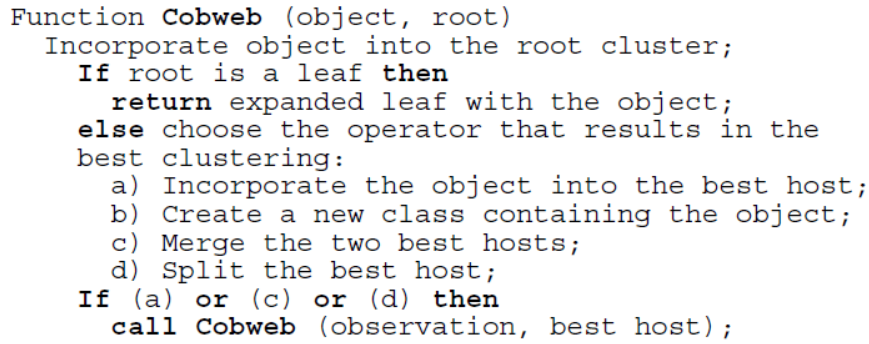
\includegraphics[scale=0.7]{img/cobweb.png}}
		\caption{Algorithme Cobweb}
	\end{figure}

\section{Les types de clusters}

Le but du clustering étant de trouver des groupes d'objets présentant des similarités
définies en fonction de l'objectif recherché. Il existe toutefois une multitude de types de cluster qui seront étudiés au sein de cette section chacun avec ses avantages et inconvénients en fonction de notre cas avant de statuer sur le type qui sera utilisé pour le reste de ce document.

\subsection{Well-Separated}
Un cluster "well-separated" est un regroupement de points de telle façon à ce que tous les points faisant parti d'un même cluster présentent de fortes similarités entre eux comparés aux points d'un cluster extérieur(figure 1.3). Si la population de cluster est suffisament bien compartimentée, ce type de cluster permet de faire fonctionner n'importe quelle méthode de clustering de façon efficace.
	\begin{figure}[h!]
		\centerline{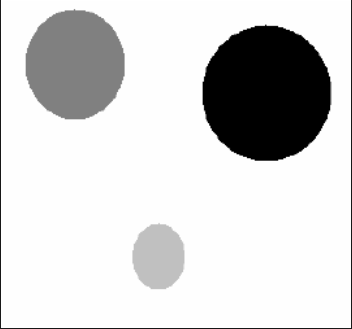
\includegraphics[scale=0.8]{img/well_separated.png}}
		\caption{Well separated clusters}
	\end{figure}

\subsection{Graph-Based}
Le graph-based cluster est utilisé dans les cas ou les données peuvent être représenté sous forme de graphe dont les nœuds sont des objets et les liens représentent les connexions entre ceux-ci. Dans cette situation un cluster peut être défini comme un composant connecté,  c'est-à-dire un groupe d'objets liés les uns aux autres au sein du même groupe. En outre ce type de classification permet de visualiser facilement d'importants jeux de données.
La théorie des graphes peut être utiliser afin d’apporter des informations plus précises sur le jeu de données en ce qui concerne les cluster, cliques et outliers. Une approche hiérarchique peut être employée à travers la création d’un arbre couvrant de poids minimal ou minimum spanning tree. Dans un contexte ou un graph G est connexe, l’arbre est un sous-graphe connexe avec un poids minimal contenant tous les nœuds du graphe d’origine G et ne possédant pas de cycle. Il existe deux algorithmes permettant d’établir ce type d’arbre, l’algorithme de Prim et l’algorithme de Kruskal.
\subsubsection{L'algorithme de Prim}
L’algorithme de Prim est un algorithme dit « glouton », c'est-à-dire qu’il va pour chaque étape effectuer un choix local jugé optimum. Cet algorithme ( figure …) va s’exécuter en choisissant un axe de poids minimal jusqu’à ce que tous les sommets aient été atteints. Il existe cependant une part d'indéterminisme, il est en effet possible que deux exécutions de cet algorithme renvoient chacun une solution différente. A noter que celle-ci sera tout de même optimale.
\newpage
\subsubsection{L’algorithme de Kruskal}
Créé en 1956  par  Joseph Kruskal  cet algorithme utilise comme entrée un graphe connexe non orienté et pondéré (figure 1.6) et va considérer chaque arrête par ordre croissant. Si l’arrête sélectionnée ne crée pas de cycle, celle-ci sera utilisée dans la construction d’un arbre couvrant de poids minimum.\\
Les algorithmes de Prim et Kruskal possédant chacun une part d’indéterminisme, il est tout à fait possible que chacun renvoie un arbre différent tout en utilisant le même graphe de départ. Les solutions données seront toutefois jugées optimales pour les deux algorithmes.
	\begin{figure}[h!]
		\centerline{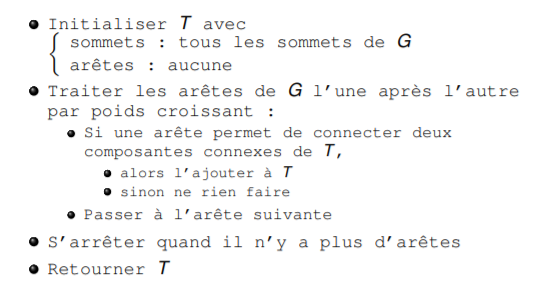
\includegraphics[scale=0.8]{img/kruskal.png}}
		\caption{Algorithme de Kruskal}
	\end{figure}
\newpage
\subsection{Density-Based}
A travers l'utilisation d'un density-based cluster, le but est de détecter les zones ou les points formant des clusters sont concentrés et celles ou les points sont séparés par des zones vides ou par des zones contenant très peu de points (figure 1.4). Les points ne faisant par partie d'un agrégat sont ici considérés comme du bruit. Ce type de définition est utilisée lorsque les clusters s'entrecroisent ou sont irréguliers.\cite{ref4} Il est également possible d'avoir recours à ce type de classification lorsque du bruit est présent, celui-ci peut former des ponts entre les clusters lorsqu'un autre type de classification est utilisée.
	\begin{figure}[h!]
		\centerline{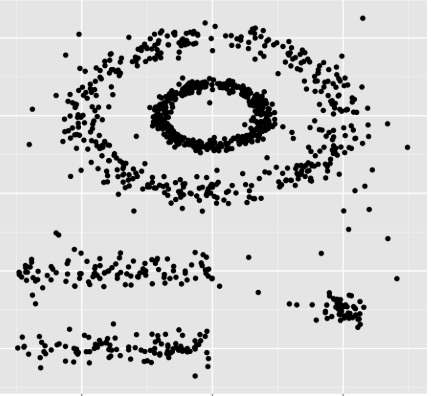
\includegraphics[scale=0.8]{img/density_cluster.png}}
		\caption{Density based clusters}
	\end{figure}

\newpage
\section{Les algorithmes}
Dans cette section seront décrit les principaux algorithmes utilisés lorsque des techniques de clustering sont employées. Les avantages et inconvénients de chacun seront présentés en fonction du cas présenté dans l'introduction.
\subsection{K-means}

L'algorithme K-means est l'algorithme le plus populaire, celui-ci peut être utiliser dans plusieurs domaines tels que : 
\begin{itemize}
\item Utilisation du clustering dans un contexte de Data Mining.
\item Clustering de documents qui dans notre cas seraient les CV d'anciens étudiants.
\item La segmentation d'un jeu de données en fonction de critères.
\end{itemize}
Celui-ci recherche la meilleure division possible au sein d'un jeux de données \cite{ref5} et possède comme avantage une certaine facilité d'implémentation. Cependant, il impose de savoir le nombre de clusters \textbf{K} souhaités et par conséquent une bonne connaissance des données utilisées. L'une des solutions possibles, lorsqu'un grand jeu de données est utilisé afin de déterminer le nombre de cluster voulu est de lancer l'algorithme avec différentes valeurs et de calculer ensuite la variance entre les résultats obtenus. Celle-ci représente ainsi la somme des distances entre chaque \textit{centroïde}.\\
K-means fonctionne de la façon suivante : 
\begin{itemize}
\item Choix d'un nombre de clusters K
\item Affectation de chaque point au groupe dont il est le plus proche.
\item Itération jusqu'à ce qu'il n'y ait plus de changements au niveau des centroïdes, c'est à dire que ceux-ci ne bougent plus lors des itérations.
\end{itemize}

\subsection{Agglomerative Hierarchical Clustering}

Les techniques de clustering agglomératives partent d'un ensemble de points formant un cluster, par la suite, les deux clusters les plus proches sont fusionnés successivement jusqu'à ce qu'il n'y est plus qu'un seul cluster restant. \cite{ref4}
\newpage
\subsection{DBSCAN}
DBSCAN est un algorithme basé sur le partitionnement de données, celui-ci utilise deux principaux paramètres qui sont la distance minimale entre deux points et le nombre de points minimum devant se trouver dans un rayon donné afin qu'ils soient considérés comme un cluster\cite{ref12}. Le choix d'une bonne mesure de la distance reste critique comme dans toute autre méthode de clustering. En effet, si la valeur choisie est trop petite, une partie des données traites risque d'être considérer des \textit {outliers} c'est à dire des observations peu fréquentes sortant de la norme.\\
l'agorithme DBSCAN sert dans des situations ou l'on cherche à déterminer des structures au sein d'un jeu de données, celui-ci peut être exprimer en peudo-code.(figure 1.5) Du à sa popularité, cet algorithme est souvent directement importé à travers des libraires Python ou R.
	\begin{figure}[h!]
		\centerline{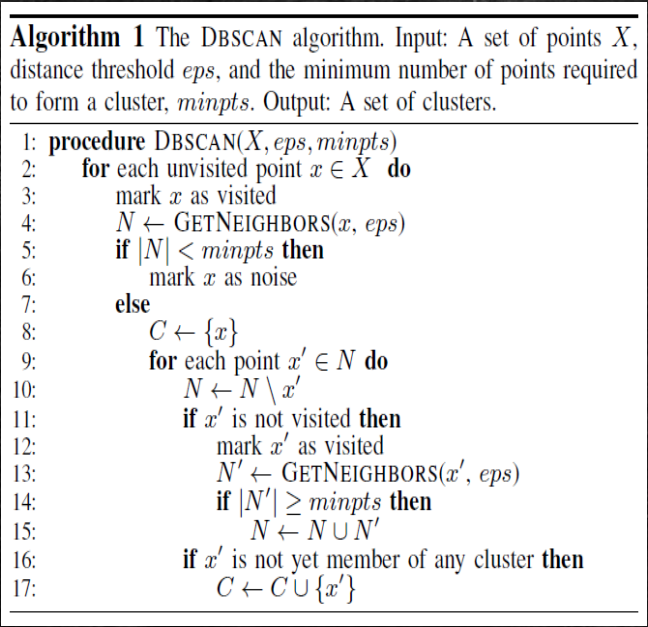
\includegraphics[scale=0.8]{img/dbscan.png}}
		\caption{Algorithme DBSCAN}
	\end{figure}
Cet algorithme offre comme avantages le fait qu'il n'a pas besoin de plus de paramètre que la distance, ici marquée \textit{eps} et le nombre de moins minimum afin de constituer un cluster représenter ici par \textit{minpts}. De plus, celui-ci n'est pas très sensible à l'ordre des données pour son traitement. Cependant, la qualité du résultat est grandement lié au choix d'une bonne mesure de distance. En outre, un degré de compréhension de l'échelle appliquée et des données étudiées est nécessaire afin de pouvoir choisir une mesure de distance pertinente.
\end{document}